% Options for packages loaded elsewhere
\PassOptionsToPackage{unicode}{hyperref}
\PassOptionsToPackage{hyphens}{url}
%
\documentclass[
  12pt,
]{article}
\usepackage{amsmath,amssymb}
\usepackage{iftex}
\ifPDFTeX
  \usepackage[T1]{fontenc}
  \usepackage[utf8]{inputenc}
  \usepackage{textcomp} % provide euro and other symbols
\else % if luatex or xetex
  \usepackage{unicode-math} % this also loads fontspec
  \defaultfontfeatures{Scale=MatchLowercase}
  \defaultfontfeatures[\rmfamily]{Ligatures=TeX,Scale=1}
\fi
\usepackage{lmodern}
\ifPDFTeX\else
  % xetex/luatex font selection
\fi
% Use upquote if available, for straight quotes in verbatim environments
\IfFileExists{upquote.sty}{\usepackage{upquote}}{}
\IfFileExists{microtype.sty}{% use microtype if available
  \usepackage[]{microtype}
  \UseMicrotypeSet[protrusion]{basicmath} % disable protrusion for tt fonts
}{}
\makeatletter
\@ifundefined{KOMAClassName}{% if non-KOMA class
  \IfFileExists{parskip.sty}{%
    \usepackage{parskip}
  }{% else
    \setlength{\parindent}{0pt}
    \setlength{\parskip}{6pt plus 2pt minus 1pt}}
}{% if KOMA class
  \KOMAoptions{parskip=half}}
\makeatother
\usepackage{xcolor}
\usepackage[margin=1in]{geometry}
\usepackage{longtable,booktabs,array}
\usepackage{calc} % for calculating minipage widths
% Correct order of tables after \paragraph or \subparagraph
\usepackage{etoolbox}
\makeatletter
\patchcmd\longtable{\par}{\if@noskipsec\mbox{}\fi\par}{}{}
\makeatother
% Allow footnotes in longtable head/foot
\IfFileExists{footnotehyper.sty}{\usepackage{footnotehyper}}{\usepackage{footnote}}
\makesavenoteenv{longtable}
\usepackage{graphicx}
\makeatletter
\def\maxwidth{\ifdim\Gin@nat@width>\linewidth\linewidth\else\Gin@nat@width\fi}
\def\maxheight{\ifdim\Gin@nat@height>\textheight\textheight\else\Gin@nat@height\fi}
\makeatother
% Scale images if necessary, so that they will not overflow the page
% margins by default, and it is still possible to overwrite the defaults
% using explicit options in \includegraphics[width, height, ...]{}
\setkeys{Gin}{width=\maxwidth,height=\maxheight,keepaspectratio}
% Set default figure placement to htbp
\makeatletter
\def\fps@figure{htbp}
\makeatother
\setlength{\emergencystretch}{3em} % prevent overfull lines
\providecommand{\tightlist}{%
  \setlength{\itemsep}{0pt}\setlength{\parskip}{0pt}}
\setcounter{secnumdepth}{5}
\newlength{\cslhangindent}
\setlength{\cslhangindent}{1.5em}
\newlength{\csllabelwidth}
\setlength{\csllabelwidth}{3em}
\newlength{\cslentryspacingunit} % times entry-spacing
\setlength{\cslentryspacingunit}{\parskip}
\newenvironment{CSLReferences}[2] % #1 hanging-ident, #2 entry spacing
 {% don't indent paragraphs
  \setlength{\parindent}{0pt}
  % turn on hanging indent if param 1 is 1
  \ifodd #1
  \let\oldpar\par
  \def\par{\hangindent=\cslhangindent\oldpar}
  \fi
  % set entry spacing
  \setlength{\parskip}{#2\cslentryspacingunit}
 }%
 {}
\usepackage{calc}
\newcommand{\CSLBlock}[1]{#1\hfill\break}
\newcommand{\CSLLeftMargin}[1]{\parbox[t]{\csllabelwidth}{#1}}
\newcommand{\CSLRightInline}[1]{\parbox[t]{\linewidth - \csllabelwidth}{#1}\break}
\newcommand{\CSLIndent}[1]{\hspace{\cslhangindent}#1}
\usepackage{xcolor}
\usepackage{float}
\usepackage{makecell}
\usepackage{multirow}
\usepackage{colortbl}
\usepackage{lscape}
\newcommand{\blandscape}{\begin{landscape}}
\newcommand{\elandscape}{\end{landscape}}
\usepackage{flafter}
\usepackage{palatino}
\renewcommand{\familydefault}{\sfdefault} % sans serif
\fontfamily{ppl}\selectfont
\ifLuaTeX
  \usepackage{selnolig}  % disable illegal ligatures
\fi
\IfFileExists{bookmark.sty}{\usepackage{bookmark}}{\usepackage{hyperref}}
\IfFileExists{xurl.sty}{\usepackage{xurl}}{} % add URL line breaks if available
\urlstyle{same}
\hypersetup{
  pdftitle={Local Authority Parking Finances in Scotland 2018-19},
  hidelinks,
  pdfcreator={LaTeX via pandoc}}

\title{Local Authority Parking Finances in Scotland 2018-19}
\author{}
\date{\vspace{-2.5em}}

\begin{document}
\maketitle

\renewcommand{\arraystretch}{1.2}

This note covers parking finances for the 32 local authorities in Scotland. They are required to submit details of their finances to the Scottish Government annually in a standard format. The figures are normally published in March, nearly a year after the financial year end. This note looks at the section on parking income and expenditure for 2014-15 to 2018-19 and is based primarily on Scottish Local Government Finance Statistics data (Scottish Government (2020)), as well as data reported by English and Welsh Local Government authorities which is used for comparison, all of the sources of which are listed in the references\footnote{Contains public sector information licensed under the \href{http://www.nationalarchives.gov.uk/doc/open-government-licence/version/3/}{Open Government Licence v3.0}.}. \emph{N.B. Aberdeen City does not publish its data in the LGF figures and therefore data has been extracted from its annual accounts where necessary (see Aberdeen City Council (2017 and 2018))}.

In addition, Transport Scotland is now publishing an annual report on decriminalised parking - the latest being: \emph{Decriminalised Parking Enforcement -- Local Authorities' Income and Expenditure:} 2018 to 2019 (Transport Scotland (2018b)), which follows on from a report \emph{released} in 2016 by the Scottish Parliament Rural Economy and Connectivity Committee that showed for the first time the number of Penalty Charge Notices (PCNs) issued and penalty income raised in Scotland for the years 2013-14 to 2015-16 (Transport Scotland (2016)).

The Transport Scotland report deals with the statutory returns which are required by councils operating Decriminalised Parking Enforcement (DPE) to show how the surpluses are reinvested in transport activities. The local finance figures also include non-DPE activities, primarily off-street parking.

\hypertarget{introduction}{%
\section{Introduction}\label{introduction}}

Table 1 shows that as of the end of 2019, 21 councils were operating DPE (using local traffic wardens and civil enforcement), while two more were actively working towards DPE. The remaining ten authorities were not currently considering DPE, but still use fixed penalty notices issued instead of fines enforced by the Justice of the Peace courts. See Figure \ref{fig:map1} for the map\footnote{Boundary data for this and all further maps is from Office for National Statistics (2017). Contains public sector information licensed under the \href{http://www.nationalarchives.gov.uk/doc/open-government-licence/version/3/}{Open Government Licence v3.0.}}.

Police Scotland no longer enforces parking offences but now deals only with dangerous parking (e.g.~on pedestrian crossings) by local arrangement. Several of the authorities not using DPE have rejected it because of the cost of setting it up and running it for the small number of parking offences.

\begingroup\fontsize{10}{12}\selectfont

\begin{longtable}[t]{lll}
\caption{\label{tab:dpe}Parking arrangements for local authorities in Scotland}\\
\toprule
Using DPE & Considering using DPE & Not using DPE\\
\midrule
\endfirsthead
\caption[]{\label{tab:dpe}Parking arrangements for local authorities in Scotland \textit{(continued)}}\\
\toprule
Using DPE & Considering using DPE & Not using DPE\\
\midrule
\endhead

\endfoot
\bottomrule
\endlastfoot
Angus (2017) & North Ayrshire & Aberdeenshire\\
Argyll and Bute (2014) & Orkney Islands & Clackmannanshire\\
Edinburgh City (1998) &  & Dumfries and Galloway\\
Dundee City (2004) &  & Moray\\
East Ayrshire (2012) &  & Na h-Eileanan an Iar\\
East Dunbartonshire (2014) &  & Scottish Borders\\
East Lothian (2017) &  & Shetland Islands\\
East Renfrewshire (2013) &  & West Dunbartonshire\\
Falkirk (2018) &  & West Lothian\\
Fife (2013) &  & \\
Glasgow City (1999) &  & \\
Highland (2016) &  & \\
Inverclyde (2014) &  & \\
Midlothian (2018) &  & \\
North Lanarkshire (2017) &  & \\
Perth and Kinross (2002) &  & \\
Renfrewshire (2010) &  & \\
South Ayrshire (2012) &  & \\
South Lanarkshire (2005) &  & \\
Stirling (2017) &  & \\
Aberdeen City (2003) &  & \\*
\end{longtable}
\endgroup{}



\begin{figure}
\centering
\includegraphics{C:/Users/TIM.CHATTERTON/OneDrive - The Royal Automobile Club Ltd/R Projects/2022-rac-parking/outputs/reports/scotland-report-2018-19_files/figure-latex/map1-1.pdf}
\caption{\label{fig:map1}Map showing implementation of decriminalised parking in Scotland (Boundary data for this map is from Office for National Statistics (2017))}
\end{figure}

\hypertarget{summary}{%
\section{Summary}\label{summary}}

Table \ref{tab:sumtab} and Figure \ref{fig:fig1} show the summary accounts for local authorities in Scotland for fiscal years 2014-15 to 2018-19. The income has
increased by 0.4\%, the expenditure has
fallen by 4.7\%, and the surplus has
increased by 5.4\%
compared to the previous fiscal year. Total transport expenditures have
fallen by 12.0\% and the surplus now represents 12.5\% of net transport expenditure. Parking makes a
smaller contribution to overall transport expenditure in Scotland compared with England where it is 24.3\% of total transport.

\newpage

\begingroup\fontsize{10}{12}\selectfont

\begin{longtable}[t]{>{\raggedleft\arraybackslash}p{3cm}>{\raggedleft\arraybackslash}p{3cm}rrrrrr}
\caption{\label{tab:sumtab}Summary of parking accounts for Scotland (£ millions)}\\
\toprule
 &  & \multirow{1}{*}[0pt]{2014-15} & \multirow{1}{*}[0pt]{2015-16} & \multirow{1}{*}[0pt]{2016-17} & \multirow{1}{*}[0pt]{2017-18} & \multirow{1}{*}[0pt]{2018-19} & \makecell[c]{Change\\2018-19\\on\\2017-18}\\
\midrule
\endfirsthead
\caption[]{\label{tab:sumtab}Summary of parking accounts for Scotland (£ millions) \textit{(continued)}}\\
\toprule
 &  & \multirow{1}{*}[0pt]{2014-15} & \multirow{1}{*}[0pt]{2015-16} & \multirow{1}{*}[0pt]{2016-17} & \multirow{1}{*}[0pt]{2017-18} & \multirow{1}{*}[0pt]{2018-19} & \makecell[c]{Change\\2018-19\\on\\2017-18}\\
\midrule
\endhead

\endfoot
\bottomrule
\endlastfoot
 & Income & 75.4 & 77.8 & 82.6 & 88.2 & 88.6 & 0.4\%\\
\nopagebreak
 & Expenditure & 39.3 & 39.6 & 40.0 & 43.6 & 41.6 & -4.7\%\\
\nopagebreak
\multirow{-3}{*}{\raggedleft\arraybackslash Parking} & Surplus & 36.1 & 38.2 & 42.6 & 44.6 & 47.0 & 5.4\%\\
\cmidrule{1-8}\pagebreak[0]
Total transport & Net expenditure & 419.6 & 439.7 & 412.9 & 426.7 & 375.3 & -12.0\%\\
\cmidrule{1-8}\pagebreak[0]
 & Parking surplus as percentage of net transport expenditure & 8.6 & 8.7 & 10.3 & 10.4 & 12.5 & \\*
\end{longtable}
\endgroup{}

\begin{figure}
\centering
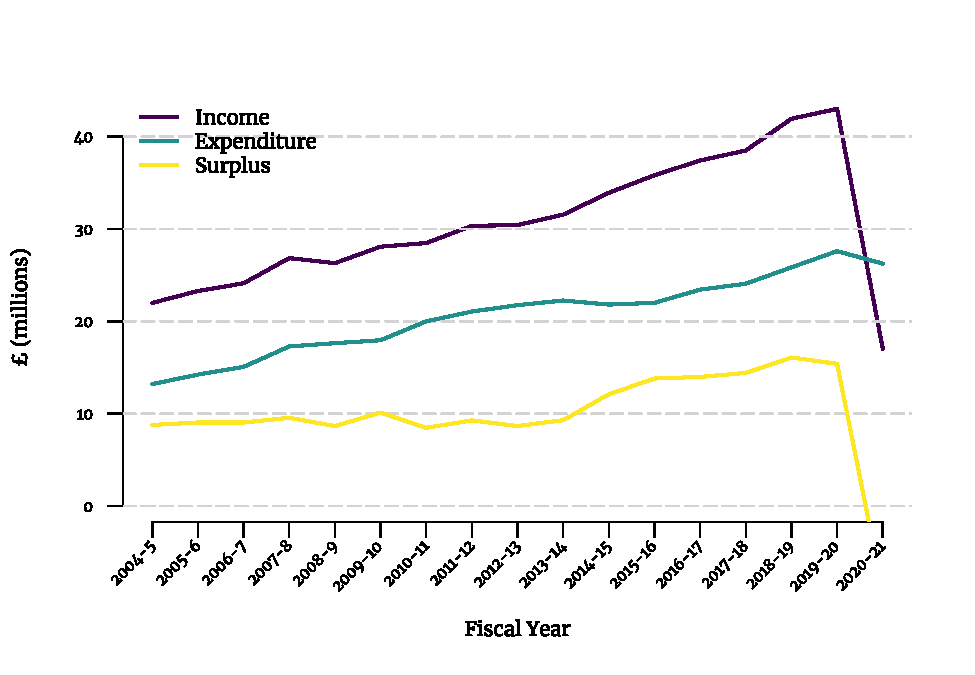
\includegraphics{C:/Users/TIM.CHATTERTON/OneDrive - The Royal Automobile Club Ltd/R Projects/2022-rac-parking/outputs/reports/scotland-report-2018-19_files/figure-latex/fig1-1.pdf}
\caption{\label{fig:fig1}Parking revenues--Scotland}
\end{figure}

Since 2014-15 income has risen by
17.5\% and expenditure has risen by 5.9\%. Over the same period the surplus has risen by 30.0\%. Figure \ref{fig:fig1} gives a longer term overview of the trends in incomes, expenditures and surpluses.

\newpage

\begingroup\fontsize{10}{12}\selectfont

\begin{longtable}[t]{rrrrrr}
\caption{\label{tab:compare}Comparison of parking income and expenditure in across the nations of Great Britain (£ millions, latest year available)}\\
\toprule
 & \makecell[c]{England\\without\\London} & London & Scotland & Wales & \makecell[c]{Great\\Britain}\\
\midrule
\endfirsthead
\caption[]{\label{tab:compare}Comparison of parking income and expenditure in across the nations of Great Britain (£ millions, latest year available) \textit{(continued)}}\\
\toprule
 & \makecell[c]{England\\without\\London} & London & Scotland & Wales & \makecell[c]{Great\\Britain}\\
\midrule
\endhead

\endfoot
\bottomrule
\endlastfoot
Fiscal year & (2018-19) & (2018-19) & (2018-19) & (2018-19) & (2018-19)\\
\midrule
Parking income & 1021.3 & 728.0 & 88.6 & 41.9 & 1879.7\\
Parking expenditure & 539.6 & 273.5 & 41.6 & -16.1 & 838.7\\
Surplus & 481.7 & 454.4 & 47.0 & 58.0 & 1041.1\\
\midrule
Surplus as proportion of income & 47.2\% & 62.4\% & 53.0\% & 138.4\% & 55.4\%\\*
\end{longtable}
\endgroup{}

Table \ref{tab:compare} provides a comparison with London, England excluding London, and Wales for the most recent available data, while Table \ref{tab:change} compares the changes between 2018-19 and the previous year, with the average annual change over the four-year period starting in 2014-15 (or the most recent four-year period for which data is available). In the last year the surpluses for Scotland have increased by 5.4\%, which is less than the average annual increase observed over the preceding four years, which was 6.8\%.

On average, parking surpluses in Great Britain have increased by about 11.7\% annually over the four years compared with 2.3\% annually for the Retail Prices Index during the same period (Office for National Statistics (2023)).

\begingroup\fontsize{10}{12}\selectfont

\begin{longtable}[t]{rrrrrr}
\caption{\label{tab:change}Changes in parking income and expenditure over previous four years (from most recent year available) across the nations of Great Britain}\\
\toprule
 & \makecell[c]{England\\without\\London} & London & Scotland & Wales & \makecell[c]{Great\\Britain}\\
\midrule
\endfirsthead
\caption[]{\label{tab:change}Changes in parking income and expenditure over previous four years (from most recent year available) across the nations of Great Britain \textit{(continued)}}\\
\toprule
 & \makecell[c]{England\\without\\London} & London & Scotland & Wales & \makecell[c]{Great\\Britain}\\
\midrule
\endhead

\endfoot
\bottomrule
\endlastfoot
Most recent year available & (2018-19) & (2018-19) & (2018-19) & (2018-19) & (2018-19)\\
\midrule
Average annual change in income & 4.3 \% & 5.8 \% & 4.1 \% & 5.4 \% & 4.9 \%\\
Change in income since previous year & 4.2 \% & 7.1 \% & 0.4 \% & 8.9 \% & 5.2 \%\\
\midrule
Average annual change in expenditure & 2.8 \% & 0.0 \% & 1.5 \% & NaN \% & 0.6 \%\\
Change in expenditure since previous year & 5.1 \% & -0.1 \% & -4.7 \% & -166.8 \% & -1.9 \%\\
\midrule
Average annual change in surplus & 6.1 \% & 10.2 \% & 6.8 \% & 48.0 \% & 9.1 \%\\
Change in surplus since previous year & 3.1 \% & 11.9 \% & 5.4 \% & 302.3 \% & 11.7 \%\\*
\end{longtable}
\endgroup{}

\newpage

\hypertarget{income}{%
\section{Income}\label{income}}

Total council parking income from all sources in Scotland for 2018-19 was £88.6 million, 0.4\% higher than 2017-18. Note that this includes meter and penalty income for on- and off-street parking, but does not include income received by private parking companies. Table \ref{tab:incometab} ranks the Scottish councils in terms of parking income.

In Scotland as a whole 22 councils increased their income over the past year and seven decreased their income. Another three councils' incomes stayed the same.
The changes from 2017-18 are mapped in Figure \ref{fig:incomefig}. The annualised changes over the previous four years are plotted in Figure \ref{fig:incomefig4}, using the same colour palette.

The top three Scottish cities by income were Edinburgh City, Glasgow City, and Aberdeen City, and between them accounted for 67.8\% of parking income.

The three councils which had the largest year-on-year percentage increases in income were East Dunbartonshire (up 91.0\%), Na h-Eileanan an Iar (up 57.4\%) and Moray (up 29.1\%).
The biggest decreases were in East Ayrshire (34.8\%), and Stirling (8.0 \%) (excluding Dumfries and Galloway, and Shetland Islands where income was under £30,000).

\begingroup\fontsize{9}{11}\selectfont

\begin{longtable}[t]{rrrrrrrr}
\caption{\label{tab:incometab}Parking income for Scotland (£,000)}\\
\toprule
\multirow{1}{*}[0pt]{Local Authority} & \multirow{1}{*}[0pt]{2014-15} & \multirow{1}{*}[0pt]{2015-16} & \multirow{1}{*}[0pt]{2016-17} & \multirow{1}{*}[0pt]{2017-18} & \multirow{1}{*}[0pt]{2018-19} & \makecell[c]{Change\\2018-19\\on\\2017-18} & \makecell[c]{Average\\annual\\change\\since\\2014-15}\\
\midrule
\endfirsthead
\caption[]{\label{tab:incometab}Parking income for Scotland (£,000) \textit{(continued)}}\\
\toprule
\multirow{1}{*}[0pt]{Local Authority} & \multirow{1}{*}[0pt]{2014-15} & \multirow{1}{*}[0pt]{2015-16} & \multirow{1}{*}[0pt]{2016-17} & \multirow{1}{*}[0pt]{2017-18} & \multirow{1}{*}[0pt]{2018-19} & \makecell[c]{Change\\2018-19\\on\\2017-18} & \makecell[c]{Average\\annual\\change\\since\\2014-15}\\
\midrule
\endhead

\endfoot
\bottomrule
\endlastfoot
Edinburgh City & 25,894 & 27,712 & 30,234 & 32,556 & 32,481 & \cellcolor{white}{ -0.2\%} & \cellcolor{white}{  5.8\%}\\
Glasgow City & 18,025 & 19,530 & 20,203 & 20,086 & 19,291 & \cellcolor{white}{ -4.0\%} & \cellcolor{white}{  1.7\%}\\
Aberdeen City & 8,730 & 8,444 & 8,040 & 8,397 & 7,869 & \cellcolor{white}{ -6.3\%} & \cellcolor{white}{ -2.6\%}\\
Dundee City & 3,876 & 4,485 & 3,751 & 5,094 & 5,140 & \cellcolor{white}{  0.9\%} & \cellcolor{white}{  7.3\%}\\
Fife & 3,302 & 2,958 & 3,467 & 3,579 & 3,814 & \cellcolor{white}{  6.6\%} & \cellcolor{white}{  3.7\%}\\
Perth and Kinross & 2,916 & 2,856 & 2,905 & 3,225 & 3,546 & \cellcolor{white}{ 10.0\%} & \cellcolor{white}{  5.0\%}\\
Highland & 1,353 & 1,519 & 1,815 & 2,251 & 2,552 & \cellcolor{white}{ 13.4\%} & \cellcolor{white}{ 17.2\%}\\
South Lanarkshire & 2,281 & 2,462 & 2,352 & 2,275 & 2,301 & \cellcolor{white}{  1.1\%} & \cellcolor{white}{  0.2\%}\\
Stirling & 2,019 & 1,671 & 1,620 & 2,218 & 2,040 & \cellcolor{white}{ -8.0\%} & \cellcolor{white}{  0.3\%}\\
East Ayrshire & 1,493 & 1,528 & 1,790 & 2,084 & 1,358 & \cellcolor{white}{-34.8\%} & \cellcolor{white}{ -2.3\%}\\
Argyll and Bute & 1,005 & 1,089 & 1,089 & 1,052 & 1,191 & \cellcolor{white}{ 13.2\%} & \cellcolor{white}{  4.3\%}\\
Renfrewshire & 1,063 & 1,066 & 1,052 & 1,021 & 1,080 & \cellcolor{white}{  5.8\%} & \cellcolor{white}{  0.4\%}\\
South Ayrshire & 775 & 0 & 1,187 & 886 & 1,009 & \cellcolor{white}{ 13.9\%} & \cellcolor{white}{  6.8\%}\\
Moray & 670 & 681 & 690 & 676 & 873 & \cellcolor{white}{ 29.1\%} & \cellcolor{white}{  6.8\%}\\
East Dunbartonshire & 54 & 53 & 184 & 323 & 617 & \cellcolor{white}{ 91.0\%} & \cellcolor{white}{ 83.9\%}\\
Falkirk & 419 & 223 & 462 & 411 & 529 & \cellcolor{white}{ 28.7\%} & \cellcolor{white}{  6.0\%}\\
Inverclyde & 157 & 328 & 385 & 396 & 507 & \cellcolor{white}{ 28.0\%} & \cellcolor{white}{ 34.1\%}\\
East Lothian & 0 & 0 & 84 & 458 & 482 & \cellcolor{white}{  5.2\%} & \cellcolor{white}{}\\
Aberdeenshire & 635 & 416 & 488 & 443 & 466 & \cellcolor{white}{  5.2\%} & \cellcolor{white}{ -7.4\%}\\
Angus & 6 & 6 & 6 & 0 & 351 & \cellcolor{white}{} & \cellcolor{white}{176.6\%}\\
East Renfrewshire & 211 & 211 & 216 & 193 & 201 & \cellcolor{white}{  4.1\%} & \cellcolor{white}{ -1.2\%}\\
North Ayrshire & 193 & 165 & 195 & 185 & 195 & \cellcolor{white}{  5.4\%} & \cellcolor{white}{  0.3\%}\\
Midlothian & 0 & 0 & 0 & 0 & 194 & \cellcolor{white}{} & \cellcolor{white}{}\\
Scottish Borders & 127 & 141 & 174 & 165 & 186 & \cellcolor{white}{ 12.7\%} & \cellcolor{white}{ 10.0\%}\\
Orkney Islands & 80 & 85 & 110 & 149 & 150 & \cellcolor{white}{  0.7\%} & \cellcolor{white}{ 17.0\%}\\
Na h-Eileanan an Iar & 38 & 37 & 36 & 47 & 74 & \cellcolor{white}{ 57.4\%} & \cellcolor{white}{ 18.1\%}\\
Clackmannanshire & 15 & 14 & 0 & 0 & 33 & \cellcolor{white}{} & \cellcolor{white}{ 21.8\%}\\
Shetland Islands & 29 & 72 & 27 & 28 & 13 & \cellcolor{white}{-53.6\%} & \cellcolor{white}{-18.2\%}\\
Dumfries and Galloway & 14 & 14 & 15 & 17 & 11 & \cellcolor{white}{-35.3\%} & \cellcolor{white}{ -5.9\%}\\
North Lanarkshire & 0 & 0 & 0 & 0 & 0 & \cellcolor{white}{  0.0\%} & \cellcolor{white}{  0.0\%}\\
West Dunbartonshire & 0 & 0 & 0 & 0 & 0 & \cellcolor{white}{  0.0\%} & \cellcolor{white}{  0.0\%}\\
West Lothian & 0 & 0 & 0 & 0 & 0 & \cellcolor{white}{  0.0\%} & \cellcolor{white}{  0.0\%}\\
\midrule
Total & 75,380 & 77,766 & 82,577 & 88,215 & 88,554 & \cellcolor{white}{  0.4\%} & \cellcolor{white}{  4.1\%}\\*
\end{longtable}
\endgroup{}

\begin{figure}
\centering
\includegraphics{C:/Users/TIM.CHATTERTON/OneDrive - The Royal Automobile Club Ltd/R Projects/2022-rac-parking/outputs/reports/scotland-report-2018-19_files/figure-latex/incomefig-1.pdf}
\caption{\label{fig:incomefig}Map of change in parking income from 2017-18 to 2018-19 (Boundary data for this map is from Office for National Statistics (2017))}
\end{figure}

Table \ref{tab:pcntab} shows the number of PCNs issued council by council in Scotland for the years 2014-15 to 2018-19, with the average income per PCN for 2018-19. The total number of PCNs has increased by around 5.1\% a year on average. The average recovery per PCN was £31.8 in 2018-19.

\begin{figure}
\centering
\includegraphics{C:/Users/TIM.CHATTERTON/OneDrive - The Royal Automobile Club Ltd/R Projects/2022-rac-parking/outputs/reports/scotland-report-2018-19_files/figure-latex/incomefig4-1.pdf}
\caption{\label{fig:incomefig4}Map of average annual change in parking income over the past four years from 2014-15 to 2018-19 (Boundary data for this map is from Office for National Statistics (2017))}
\end{figure}

\newpage

\pagebreak

\begingroup\fontsize{10}{12}\selectfont

\begin{longtable}[t]{rrrrrrr}
\caption{\label{tab:pcntab}Number of PCNs for councils using DPE and average 2018-19 income per PCN}\\
\toprule
\multirow{1}{*}[0pt]{Local Authority} & \multirow{1}{*}[0pt]{2014-15} & \multirow{1}{*}[0pt]{2015-16} & \multirow{1}{*}[0pt]{2016-17} & \multirow{1}{*}[0pt]{2017-18} & \multirow{1}{*}[0pt]{2018-19} & \makecell[c]{£/PCN\\(2018-19)}\\
\midrule
\endfirsthead
\caption[]{\label{tab:pcntab}Number of PCNs for councils using DPE and average 2018-19 income per PCN \textit{(continued)}}\\
\toprule
\multirow{1}{*}[0pt]{Local Authority} & \multirow{1}{*}[0pt]{2014-15} & \multirow{1}{*}[0pt]{2015-16} & \multirow{1}{*}[0pt]{2016-17} & \multirow{1}{*}[0pt]{2017-18} & \multirow{1}{*}[0pt]{2018-19} & \makecell[c]{£/PCN\\(2018-19)}\\
\midrule
\endhead

\endfoot
\bottomrule
\endlastfoot
Aberdeen City & 46,450 & 37,754 & 37,754 & 40,392 & 38,967 & £35.5\\
Angus &  &  &  & 6,273 & 6,626 & £30.9\\
Argyll and Bute & 5,929 & 8,123 & 13,018 & 6,269 & 6,696 & £31.4\\
Dundee City & 25,415 & 31,332 & 29,266 & 21,837 & 29,130 & £30.3\\
East Ayrshire & 6,232 & 5,391 & 5,995 & 6,262 & 6,900 & £41.6\\
East Dunbartonshire & 3,948 & 3,331 & 4,704 & 5,301 & 6,348 & £34.0\\
East Lothian &  &  & 953 & 10,040 & 9,540 & £33.1\\
East Renfrewshire & 4,322 & 5,696 & 3,742 & 5,176 & 4,859 & £38.5\\
Edinburgh City & 179,340 & 184,964 & 192,381 & 191,563 & 183,965 & £28.8\\
Falkirk &  &  &  &  & 2,881 & £19.9\\
Fife & 19,248 & 19,904 & 20,142 & 21,890 & 21,768 & £27.8\\
Glasgow City & 116,937 & 118,902 & 133,901 & 125,505 & 146,412 & £34.3\\
Highland &  &  & 4,101 & 9,477 & 10,000 & £30.7\\
Inverclyde & 3,439 & 6,260 & 7,200 & 8,059 & 9,117 & £45.2\\
Midlothian &  &  &  &  & 6,855 & £23.5\\
North Lanarkshire &  &  &  &  & 6,018 & £25.0\\
Perth and Kinross & 9,077 & 7,133 & 7,805 & 14,469 & 15,852 & £37.1\\
Renfrewshire & 7,497 & 7,588 & 6,160 & 6,823 & 6,974 & £23.5\\
South Ayrshire & 6,716 & 5,968 & 5,238 & 5,824 & 7,213 & £31.2\\
South Lanarkshire & 22,412 & 23,513 & 23,693 & 20,952 & 21,281 & £34.1\\
Stirling &  &  &  & 9,975 & 9,586 & £30.7\\
\midrule
Total & 456,962 & 465,859 & 496,053 & 516,087 & 556,988 & £31.8\\*
\end{longtable}
\endgroup{}
\newpage
\begingroup\fontsize{10}{12}\selectfont

\begin{longtable}[t]{rrrrrr}
\caption{\label{tab:pcnprop}Proportion of parking income from PCNs in Scottish councils using DPE with London, and England excluding London, for comparison}\\
\toprule
\multirow{1}{*}[0pt]{Local Authority} & \multirow{1}{*}[0pt]{2014-15} & \multirow{1}{*}[0pt]{2015-16} & \multirow{1}{*}[0pt]{2016-17} & \multirow{1}{*}[0pt]{2017-18} & \multirow{1}{*}[0pt]{2018-19}\\
\midrule
\endfirsthead
\caption[]{\label{tab:pcnprop}Proportion of parking income from PCNs in Scottish councils using DPE with London, and England excluding London, for comparison \textit{(continued)}}\\
\toprule
\multirow{1}{*}[0pt]{Local Authority} & \multirow{1}{*}[0pt]{2014-15} & \multirow{1}{*}[0pt]{2015-16} & \multirow{1}{*}[0pt]{2016-17} & \multirow{1}{*}[0pt]{2017-18} & \multirow{1}{*}[0pt]{2018-19}\\
\midrule
\endhead

\endfoot
\bottomrule
\endlastfoot
Aberdeen City & \cellcolor{white}{18.8\%} & \cellcolor{white}{17.5\%} & \cellcolor{white}{20.1\%} & \cellcolor{white}{20.7\%} & \cellcolor{white}{17.6\%}\\
Argyll and Bute & \cellcolor{white}{23.2\%} & \cellcolor{white}{24.6\%} & \cellcolor{white}{38.3\%} & \cellcolor{white}{17.8\%} & \cellcolor{white}{17.7\%}\\
Dundee City & \cellcolor{white}{19.3\%} & \cellcolor{white}{24.8\%} & \cellcolor{white}{27.0\%} & \cellcolor{white}{24.9\%} & \cellcolor{white}{17.1\%}\\
East Ayrshire & \cellcolor{white}{16.8\%} & \cellcolor{white}{13.4\%} & \cellcolor{white}{13.8\%} & \cellcolor{white}{10.4\%} & \cellcolor{white}{21.1\%}\\
East Dunbartonshire & \cellcolor{white}{} & \cellcolor{white}{} & \cellcolor{white}{77.9\%} & \cellcolor{white}{53.1\%} & \cellcolor{white}{35.0\%}\\
East Lothian & \cellcolor{white}{} & \cellcolor{white}{} & \cellcolor{white}{33.5\%} & \cellcolor{white}{60.9\%} & \cellcolor{white}{65.5\%}\\
East Renfrewshire & \cellcolor{white}{99.2\%} & \cellcolor{white}{98.8\%} & \cellcolor{white}{97.9\%} & \cellcolor{white}{98.7\%} & \cellcolor{white}{93.0\%}\\
Edinburgh City & \cellcolor{white}{19.8\%} & \cellcolor{white}{18.9\%} & \cellcolor{white}{18.6\%} & \cellcolor{white}{18.1\%} & \cellcolor{white}{16.3\%}\\
Fife & \cellcolor{white}{17.7\%} & \cellcolor{white}{16.9\%} & \cellcolor{white}{17.7\%} & \cellcolor{white}{16.4\%} & \cellcolor{white}{15.9\%}\\
Glasgow City & \cellcolor{white}{24.1\%} & \cellcolor{white}{20.4\%} & \cellcolor{white}{23.8\%} & \cellcolor{white}{22.0\%} & \cellcolor{white}{26.0\%}\\
Highland & \cellcolor{white}{} & \cellcolor{white}{} & \cellcolor{white}{ 3.9\%} & \cellcolor{white}{11.8\%} & \cellcolor{white}{12.0\%}\\
Inverclyde & \cellcolor{white}{84.4\%} & \cellcolor{white}{84.6\%} & \cellcolor{white}{81.5\%} & \cellcolor{white}{70.5\%} & \cellcolor{white}{81.3\%}\\
Perth and Kinross & \cellcolor{white}{11.9\%} & \cellcolor{white}{10.4\%} & \cellcolor{white}{10.8\%} & \cellcolor{white}{16.0\%} & \cellcolor{white}{16.6\%}\\
Renfrewshire & \cellcolor{white}{21.9\%} & \cellcolor{white}{20.4\%} & \cellcolor{white}{15.5\%} & \cellcolor{white}{17.6\%} & \cellcolor{white}{15.2\%}\\
South Ayrshire & \cellcolor{white}{33.0\%} & \cellcolor{white}{} & \cellcolor{white}{16.7\%} & \cellcolor{white}{21.8\%} & \cellcolor{white}{22.3\%}\\
South Lanarkshire & \cellcolor{white}{31.9\%} & \cellcolor{white}{30.3\%} & \cellcolor{white}{32.1\%} & \cellcolor{white}{30.7\%} & \cellcolor{white}{31.5\%}\\
Scottish DPE authorties & \cellcolor{white}{19.7\%} & \cellcolor{white}{19.0\%} & \cellcolor{white}{20.0\%} & \cellcolor{white}{20.0\%} & \cellcolor{white}{20.0\%}\\
London & \cellcolor{white}{40.4\%} & \cellcolor{white}{49.3\%} & \cellcolor{white}{42.0\%} & \cellcolor{white}{43.1\%} & \cellcolor{white}{45.1\%}\\
England without London & \cellcolor{white}{10.9\%} & \cellcolor{white}{11.5\%} & \cellcolor{white}{12.8\%} & \cellcolor{white}{13.8\%} & \cellcolor{white}{12.3\%}\\*
\end{longtable}
\endgroup{}

Scottish councils with DPE earn 17.6\% of their income from PCNs (see Table \ref{tab:pcnprop}).

\hypertarget{expenditure}{%
\section{Expenditure}\label{expenditure}}

\begin{figure}
\centering
\includegraphics{C:/Users/TIM.CHATTERTON/OneDrive - The Royal Automobile Club Ltd/R Projects/2022-rac-parking/outputs/reports/scotland-report-2018-19_files/figure-latex/expendfig-1.pdf}
\caption{\label{fig:expendfig}Map of change in parking expenditure from 2017-18 to 2018-19 (Boundary data for this map is from Office for National Statistics (2017))}
\end{figure}

Table \ref{tab:expendtab} ranks the councils in terms of expenditure on parking.

Overall expenditure has fallen by £2.1 million (4.7\%) after a rise of £3.7 million last year.

In Scotland as a whole 16 councils increased their expenditures over the past year and 15 decreased them. Another single council's expenditure stayed the same. The changes from 2017-18 are mapped in Figure \ref{fig:expendfig}. The average annual changes over the previous four years are plotted in Figure \ref{fig:expendfig4}, using the same colour palette.

The largest increase in expenditure occured in Midlothian where it increased by 69.7\%
while Shetland Islands and Renfrewshire increased by 37.5\% and 35.8\% respectively. The biggest decreases were in East Ayrshire (42.5\%), and Moray (19.4 \%).

The table also shows the proportion of income taken up by costs in 2018-19. Nationally in Scotland it is 47.0\% with Glasgow at 33.6\% and Edinburgh at 25.9\%.

\begingroup\fontsize{8}{10}\selectfont

\begin{longtable}[t]{rrrrrrrrr}
\caption{\label{tab:expendtab}Parking expenditure for Scotland (£,000)}\\
\toprule
\multirow{1}{*}[0pt]{Local Authority} & \multirow{1}{*}[0pt]{2014-15} & \multirow{1}{*}[0pt]{2015-16} & \multirow{1}{*}[0pt]{2016-17} & \multirow{1}{*}[0pt]{2017-18} & \multirow{1}{*}[0pt]{2018-19} & \makecell[c]{Change\\2018-19\\on\\2017-18} & \makecell[c]{Average\\annual\\change\\since\\2014-15} & \makecell[c]{Expenditure\\as\\proportion\\of income}\\
\midrule
\endfirsthead
\caption[]{\label{tab:expendtab}Parking expenditure for Scotland (£,000) \textit{(continued)}}\\
\toprule
\multirow{1}{*}[0pt]{Local Authority} & \multirow{1}{*}[0pt]{2014-15} & \multirow{1}{*}[0pt]{2015-16} & \multirow{1}{*}[0pt]{2016-17} & \multirow{1}{*}[0pt]{2017-18} & \multirow{1}{*}[0pt]{2018-19} & \makecell[c]{Change\\2018-19\\on\\2017-18} & \makecell[c]{Average\\annual\\change\\since\\2014-15} & \makecell[c]{Expenditure\\as\\proportion\\of income}\\
\midrule
\endhead

\endfoot
\bottomrule
\endlastfoot
Edinburgh City & 8,539 & 8,355 & 8,365 & 8,737 & 8,399 & \cellcolor{white}{ -3.9\%} & \cellcolor{white}{ -0.4\%} & 25.9\%\\
Glasgow City & 6,670 & 6,948 & 6,952 & 7,544 & 6,490 & \cellcolor{white}{-14.0\%} & \cellcolor{white}{ -0.7\%} & 33.6\%\\
Aberdeen City & 4,221 & 4,877 & 4,821 & 5,075 & 4,981 & \cellcolor{white}{ -1.9\%} & \cellcolor{white}{  4.2\%} & 63.3\%\\
Fife & 3,003 & 2,779 & 3,013 & 3,204 & 3,306 & \cellcolor{white}{  3.2\%} & \cellcolor{white}{  2.4\%} & 86.7\%\\
Dundee City & 2,681 & 2,840 & 2,848 & 3,401 & 3,018 & \cellcolor{white}{-11.3\%} & \cellcolor{white}{  3.0\%} & 58.7\%\\
Perth and Kinross & 2,245 & 2,635 & 2,395 & 2,499 & 2,668 & \cellcolor{white}{  6.8\%} & \cellcolor{white}{  4.4\%} & 75.2\%\\
Stirling & 1,880 & 1,508 & 1,546 & 1,693 & 1,661 & \cellcolor{white}{ -1.9\%} & \cellcolor{white}{ -3.0\%} & 81.4\%\\
South Lanarkshire & 1,674 & 1,832 & 1,696 & 1,502 & 1,560 & \cellcolor{white}{  3.9\%} & \cellcolor{white}{ -1.7\%} & 67.8\%\\
Highland & 950 & 1,119 & 1,334 & 1,607 & 1,422 & \cellcolor{white}{-11.5\%} & \cellcolor{white}{ 10.6\%} & 55.7\%\\
East Ayrshire & 1,241 & 962 & 955 & 1,698 & 977 & \cellcolor{white}{-42.5\%} & \cellcolor{white}{ -5.8\%} & 71.9\%\\
Argyll and Bute & 679 & 726 & 726 & 705 & 834 & \cellcolor{white}{ 18.3\%} & \cellcolor{white}{  5.3\%} & 70.0\%\\
Aberdeenshire & 505 & 568 & 589 & 625 & 645 & \cellcolor{white}{  3.2\%} & \cellcolor{white}{  6.3\%} & 138.4\%\\
Renfrewshire & 540 & 368 & 289 & 424 & 576 & \cellcolor{white}{ 35.8\%} & \cellcolor{white}{  1.6\%} & 53.3\%\\
East Dunbartonshire & 384 & 549 & 341 & 513 & 535 & \cellcolor{white}{  4.3\%} & \cellcolor{white}{  8.6\%} & 86.7\%\\
South Ayrshire & 529 & 470 & 706 & 579 & 505 & \cellcolor{white}{-12.8\%} & \cellcolor{white}{ -1.2\%} & 50.0\%\\
East Lothian & 0 & 0 & 170 & 463 & 483 & \cellcolor{white}{  4.3\%} & \cellcolor{white}{} & 100.2\%\\
Inverclyde & 250 & 297 & 346 & 397 & 463 & \cellcolor{white}{ 16.6\%} & \cellcolor{white}{ 16.7\%} & 91.3\%\\
North Ayrshire & 859 & 279 & 336 & 437 & 399 & \cellcolor{white}{ -8.7\%} & \cellcolor{white}{-17.4\%} & 204.6\%\\
East Renfrewshire & 288 & 378 & 345 & 336 & 365 & \cellcolor{white}{  8.6\%} & \cellcolor{white}{  6.1\%} & 181.6\%\\
Midlothian & 94 & 135 & 229 & 211 & 358 & \cellcolor{white}{ 69.7\%} & \cellcolor{white}{ 39.7\%} & 184.5\%\\
Moray & 433 & 425 & 362 & 434 & 350 & \cellcolor{white}{-19.4\%} & \cellcolor{white}{ -5.2\%} & 40.1\%\\
Scottish Borders & 364 & 349 & 390 & 387 & 333 & \cellcolor{white}{-14.0\%} & \cellcolor{white}{ -2.2\%} & 179.0\%\\
Falkirk & 365 & 223 & 320 & 275 & 324 & \cellcolor{white}{ 17.8\%} & \cellcolor{white}{ -2.9\%} & 61.2\%\\
Dumfries and Galloway & 216 & 248 & 210 & 213 & 200 & \cellcolor{white}{ -6.1\%} & \cellcolor{white}{ -1.9\%} & 1818.2\%\\
West Lothian & 105 & 143 & 149 & 144 & 173 & \cellcolor{white}{ 20.1\%} & \cellcolor{white}{ 13.3\%} & \\
Angus & 133 & 114 & 190 & 159 & 139 & \cellcolor{white}{-12.6\%} & \cellcolor{white}{  1.1\%} & 39.6\%\\
Orkney Islands & 90 & 98 & 134 & 134 & 136 & \cellcolor{white}{  1.5\%} & \cellcolor{white}{ 10.9\%} & 90.7\%\\
Na h-Eileanan an Iar & 86 & 93 & 102 & 130 & 115 & \cellcolor{white}{-11.5\%} & \cellcolor{white}{  7.5\%} & 155.4\%\\
West Dunbartonshire & 90 & 86 & 77 & 98 & 91 & \cellcolor{white}{ -7.1\%} & \cellcolor{white}{  0.3\%} & \\
Clackmannanshire & 112 & 92 & 0 & 0 & 43 & \cellcolor{white}{} & \cellcolor{white}{-21.3\%} & 130.3\%\\
Shetland Islands & 28 & 71 & 36 & 24 & 33 & \cellcolor{white}{ 37.5\%} & \cellcolor{white}{  4.2\%} & 253.8\%\\
North Lanarkshire & 0 & 0 & 0 & 0 & 0 & \cellcolor{white}{  0.0\%} & \cellcolor{white}{  0.0\%} & 100.0\%\\
\midrule
Total & 39,254 & 39,567 & 39,972 & 43,648 & 41,582 & \cellcolor{white}{ -4.7\%} & \cellcolor{white}{  1.5\%} & 47.0\%\\*
\end{longtable}
\endgroup{}

\begin{figure}
\centering
\includegraphics{C:/Users/TIM.CHATTERTON/OneDrive - The Royal Automobile Club Ltd/R Projects/2022-rac-parking/outputs/reports/scotland-report-2018-19_files/figure-latex/expendfig4-1.pdf}
\caption{\label{fig:expendfig4}Map of average annual change in parking expenditure over the past four years from 2014-15 to 2018-19 (Boundary data for this map is from Office for National Statistics (2017))}
\end{figure}

Table \ref{tab:expendprop} shows the proportion of income taken up by expenditure over the previous four years. Across Scotland it was 47.0\% compared to 49.5\% in the previous year.

Edinburgh's expenditure was 25.9\% having fallen since last year, and Glasgow's has fallen to 33.6\%. Care should be taken in interpreting the percentages towards the bottom of the table, as the very low parking incomes can lead to extreme values which are less meaningful.

\begingroup\fontsize{10}{12}\selectfont

\begin{longtable}[t]{rrrrrr}
\caption{\label{tab:expendprop}Parking expenditure as proportion of parking income}\\
\toprule
\multirow{1}{*}[0pt]{Local Authority} & \multirow{1}{*}[0pt]{2014-15} & \multirow{1}{*}[0pt]{2015-16} & \multirow{1}{*}[0pt]{2016-17} & \multirow{1}{*}[0pt]{2017-18} & \multirow{1}{*}[0pt]{2018-19}\\
\midrule
\endfirsthead
\caption[]{\label{tab:expendprop}Parking expenditure as proportion of parking income \textit{(continued)}}\\
\toprule
\multirow{1}{*}[0pt]{Local Authority} & \multirow{1}{*}[0pt]{2014-15} & \multirow{1}{*}[0pt]{2015-16} & \multirow{1}{*}[0pt]{2016-17} & \multirow{1}{*}[0pt]{2017-18} & \multirow{1}{*}[0pt]{2018-19}\\
\midrule
\endhead

\endfoot
\bottomrule
\multicolumn{6}{l}{\rule{0pt}{1em}\textsuperscript{*} Empty cells indicate the council reported no income and/or no expenditure}\\
\endlastfoot
Edinburgh City & \cellcolor{white}{  33.0\%} & \cellcolor{white}{  30.1\%} & \cellcolor{white}{  27.7\%} & \cellcolor{white}{  26.8\%} & \cellcolor{white}{  25.9\%}\\
Glasgow City & \cellcolor{white}{  37.0\%} & \cellcolor{white}{  35.6\%} & \cellcolor{white}{  34.4\%} & \cellcolor{white}{  37.6\%} & \cellcolor{white}{  33.6\%}\\
Aberdeen City & \cellcolor{white}{  48.4\%} & \cellcolor{white}{  57.8\%} & \cellcolor{white}{  60.0\%} & \cellcolor{white}{  60.4\%} & \cellcolor{white}{  63.3\%}\\
Fife & \cellcolor{white}{  90.9\%} & \cellcolor{white}{  93.9\%} & \cellcolor{white}{  86.9\%} & \cellcolor{white}{  89.5\%} & \cellcolor{white}{  86.7\%}\\
Dundee City & \cellcolor{white}{  69.2\%} & \cellcolor{white}{  63.3\%} & \cellcolor{white}{  75.9\%} & \cellcolor{white}{  66.8\%} & \cellcolor{white}{  58.7\%}\\
Perth and Kinross & \cellcolor{white}{  77.0\%} & \cellcolor{white}{  92.3\%} & \cellcolor{white}{  82.4\%} & \cellcolor{white}{  77.5\%} & \cellcolor{white}{  75.2\%}\\
Stirling & \cellcolor{white}{  93.1\%} & \cellcolor{white}{  90.2\%} & \cellcolor{white}{  95.4\%} & \cellcolor{white}{  76.3\%} & \cellcolor{white}{  81.4\%}\\
South Lanarkshire & \cellcolor{white}{  73.4\%} & \cellcolor{white}{  74.4\%} & \cellcolor{white}{  72.1\%} & \cellcolor{white}{  66.0\%} & \cellcolor{white}{  67.8\%}\\
Highland & \cellcolor{white}{  70.2\%} & \cellcolor{white}{  73.7\%} & \cellcolor{white}{  73.5\%} & \cellcolor{white}{  71.4\%} & \cellcolor{white}{  55.7\%}\\
East Ayrshire & \cellcolor{white}{  83.1\%} & \cellcolor{white}{  63.0\%} & \cellcolor{white}{  53.4\%} & \cellcolor{white}{  81.5\%} & \cellcolor{white}{  71.9\%}\\
Argyll and Bute & \cellcolor{white}{  67.6\%} & \cellcolor{white}{  66.7\%} & \cellcolor{white}{  66.7\%} & \cellcolor{white}{  67.0\%} & \cellcolor{white}{  70.0\%}\\
Aberdeenshire & \cellcolor{white}{  79.5\%} & \cellcolor{white}{ 136.5\%} & \cellcolor{white}{ 120.7\%} & \cellcolor{white}{ 141.1\%} & \cellcolor{white}{ 138.4\%}\\
Renfrewshire & \cellcolor{white}{  50.8\%} & \cellcolor{white}{  34.5\%} & \cellcolor{white}{  27.5\%} & \cellcolor{white}{  41.5\%} & \cellcolor{white}{  53.3\%}\\
East Dunbartonshire & \cellcolor{white}{ 711.1\%} & \cellcolor{white}{1035.8\%} & \cellcolor{white}{ 185.3\%} & \cellcolor{white}{ 158.8\%} & \cellcolor{white}{  86.7\%}\\
South Ayrshire & \cellcolor{white}{  68.3\%} & \cellcolor{white}{} & \cellcolor{white}{  59.5\%} & \cellcolor{white}{  65.3\%} & \cellcolor{white}{  50.0\%}\\
East Lothian & \cellcolor{white}{} & \cellcolor{white}{} & \cellcolor{white}{ 202.4\%} & \cellcolor{white}{ 101.1\%} & \cellcolor{white}{ 100.2\%}\\
Inverclyde & \cellcolor{white}{ 159.2\%} & \cellcolor{white}{  90.5\%} & \cellcolor{white}{  89.9\%} & \cellcolor{white}{ 100.3\%} & \cellcolor{white}{  91.3\%}\\
North Ayrshire & \cellcolor{white}{ 445.1\%} & \cellcolor{white}{ 169.1\%} & \cellcolor{white}{ 172.3\%} & \cellcolor{white}{ 236.2\%} & \cellcolor{white}{ 204.6\%}\\
East Renfrewshire & \cellcolor{white}{ 136.5\%} & \cellcolor{white}{ 179.1\%} & \cellcolor{white}{ 159.7\%} & \cellcolor{white}{ 174.1\%} & \cellcolor{white}{ 181.6\%}\\
Midlothian & \cellcolor{white}{} & \cellcolor{white}{} & \cellcolor{white}{} & \cellcolor{white}{} & \cellcolor{white}{ 184.5\%}\\
Moray & \cellcolor{white}{  64.6\%} & \cellcolor{white}{  62.4\%} & \cellcolor{white}{  52.5\%} & \cellcolor{white}{  64.2\%} & \cellcolor{white}{  40.1\%}\\
Scottish Borders & \cellcolor{white}{ 286.6\%} & \cellcolor{white}{ 247.5\%} & \cellcolor{white}{ 224.1\%} & \cellcolor{white}{ 234.5\%} & \cellcolor{white}{ 179.0\%}\\
Falkirk & \cellcolor{white}{  87.1\%} & \cellcolor{white}{ 100.0\%} & \cellcolor{white}{  69.3\%} & \cellcolor{white}{  66.9\%} & \cellcolor{white}{  61.2\%}\\
Dumfries and Galloway & \cellcolor{white}{1542.9\%} & \cellcolor{white}{1771.4\%} & \cellcolor{white}{1400.0\%} & \cellcolor{white}{1252.9\%} & \cellcolor{white}{1818.2\%}\\
West Lothian & \cellcolor{white}{} & \cellcolor{white}{} & \cellcolor{white}{} & \cellcolor{white}{} & \cellcolor{white}{}\\
Angus & \cellcolor{white}{2216.7\%} & \cellcolor{white}{1900.0\%} & \cellcolor{white}{3166.7\%} & \cellcolor{white}{} & \cellcolor{white}{  39.6\%}\\
Orkney Islands & \cellcolor{white}{ 112.5\%} & \cellcolor{white}{ 115.3\%} & \cellcolor{white}{ 121.8\%} & \cellcolor{white}{  89.9\%} & \cellcolor{white}{  90.7\%}\\
Na h-Eileanan an Iar & \cellcolor{white}{ 226.3\%} & \cellcolor{white}{ 251.4\%} & \cellcolor{white}{ 283.3\%} & \cellcolor{white}{ 276.6\%} & \cellcolor{white}{ 155.4\%}\\
West Dunbartonshire & \cellcolor{white}{} & \cellcolor{white}{} & \cellcolor{white}{} & \cellcolor{white}{} & \cellcolor{white}{}\\
Clackmannanshire & \cellcolor{white}{ 746.7\%} & \cellcolor{white}{ 657.1\%} & \cellcolor{white}{} & \cellcolor{white}{} & \cellcolor{white}{ 130.3\%}\\
Shetland Islands & \cellcolor{white}{  96.6\%} & \cellcolor{white}{  98.6\%} & \cellcolor{white}{ 133.3\%} & \cellcolor{white}{  85.7\%} & \cellcolor{white}{ 253.8\%}\\
North Lanarkshire & \cellcolor{white}{} & \cellcolor{white}{} & \cellcolor{white}{} & \cellcolor{white}{} & \cellcolor{white}{}\\
\midrule
Total & \cellcolor{white}{  52.1\%} & \cellcolor{white}{  50.9\%} & \cellcolor{white}{  48.4\%} & \cellcolor{white}{  49.5\%} & \cellcolor{white}{  47.0\%}\\*
\end{longtable}
\endgroup{}

\newpage

\hypertarget{surpluses}{%
\section{Surpluses}\label{surpluses}}

Table \ref{tab:surplustab} shows the parking surpluses from 2014-15 to 2018-19 and the change from 2017-18 to 2018-19. It also shows the proportion that parking surpluses represent of total transport expenditure.

The total \emph{surpluses} for Scotland amounted to £48.4 million between 20 authorities, of which the top three--Edinburgh City, Glasgow City, and Aberdeen City--accounted for 82.2\%. 12 councils made a loss with the total of parking deficits falling to £1.4 million from £1.9 million last year.

Overall, parking contributed £47.0 million to local authority finances in Scotland in 2018-19 compared with £44.6 million in 2017-18, an increase of 5.4\%.

Moray increased their surplus by 116.1\%
while Highland and South Ayrshire increased by 75.5\% and 64.2\% respectively. The biggest decreases were in Stirling (27.8\%), and Renfrewshire (15.6 \%).

West Lothian increased their deficits by 20.1\% while East Renfrewshire and Aberdeenshire increased by 14.7\% and -1.6\% respectively The biggest decreases were in Na h-Eileanan an Iar (50.6\%), and Scottish Borders (33.8\%) (excluding East Lothian with a deficit under £30,000)

\newpage
\begingroup\fontsize{10}{12}\selectfont

\begin{longtable}[t]{rrrrrrrr}
\caption{\label{tab:surplustab}Parking surpluses for Scotland (£,000)}\\
\toprule
\multirow{1}{*}[0pt]{Local Authority} & \multirow{1}{*}[0pt]{2014-15} & \multirow{1}{*}[0pt]{2015-16} & \multirow{1}{*}[0pt]{2016-17} & \multirow{1}{*}[0pt]{2017-18} & \multirow{1}{*}[0pt]{2018-19} & \makecell[c]{Change 2018-19\\on\\2017-18} & \makecell[c]{Surplus\\as\\proportion\\of\\transport\\spending}\\
\midrule
\endfirsthead
\caption[]{\label{tab:surplustab}Parking surpluses for Scotland (£,000) \textit{(continued)}}\\
\toprule
\multirow{1}{*}[0pt]{Local Authority} & \multirow{1}{*}[0pt]{2014-15} & \multirow{1}{*}[0pt]{2015-16} & \multirow{1}{*}[0pt]{2016-17} & \multirow{1}{*}[0pt]{2017-18} & \multirow{1}{*}[0pt]{2018-19} & \makecell[c]{Change 2018-19\\on\\2017-18} & \makecell[c]{Surplus\\as\\proportion\\of\\transport\\spending}\\
\midrule
\endhead

\endfoot
\bottomrule
\multicolumn{8}{l}{\rule{0pt}{1em}\textsuperscript{*} Where the change in surplus is actually a change in deficit, the values are in italics}\\
\endlastfoot
Edinburgh City & 17,355 & 19,357 & 21,869 & 23,819 & 24,082 & 1.1\% & -265.9\%\\
Glasgow City & 11,355 & 12,582 & 13,251 & 12,542 & 12,801 & 2.1\% & 59.0\%\\
Aberdeen City & 4,509 & 3,567 & 3,219 & 3,322 & 2,888 & -13.1\% & 33.4\%\\
Dundee City & 1,195 & 1,645 & 903 & 1,693 & 2,122 & 25.3\% & 41.3\%\\
Highland & 403 & 400 & 481 & 644 & 1,130 & 75.5\% & 3.4\%\\
Perth and Kinross & 671 & 221 & 510 & 726 & 878 & 20.9\% & 7.7\%\\
South Lanarkshire & 607 & 630 & 656 & 773 & 741 & -4.1\% & 3.1\%\\
Moray & 237 & 256 & 328 & 242 & 523 & 116.1\% & 9.6\%\\
Fife & 299 & 179 & 454 & 375 & 508 & 35.5\% & 1.8\%\\
Renfrewshire & 523 & 698 & 763 & 597 & 504 & -15.6\% & 3.9\%\\
South Ayrshire & 246 & -470 & 481 & 307 & 504 & 64.2\% & 5.4\%\\
East Ayrshire & 252 & 566 & 835 & 386 & 381 & -1.3\% & 3.4\%\\
Stirling & 139 & 163 & 74 & 525 & 379 & -27.8\% & 4.6\%\\
Argyll and Bute & 326 & 363 & 363 & 347 & 357 & 2.9\% & 2.6\%\\
Angus & -127 & -108 & -184 & -159 & 212 &  & 2.0\%\\
Falkirk & 54 & 0 & 142 & 136 & 205 & 50.7\% & 2.3\%\\
East Dunbartonshire & -330 & -496 & -157 & -190 & 82 &  & 1.1\%\\
Inverclyde & -93 & 31 & 39 & -1 & 44 &  & 0.9\%\\
Orkney Islands & -10 & -13 & -24 & 15 & 14 & -6.7\% & 0.1\%\\
North Lanarkshire & 0 & 0 & 0 & 0 & 0 & 0.0\% & 0.0\%\\
East Lothian & 0 & 0 & -86 & -5 & -1 & \em{-80.0\%} & 0.0\%\\
Clackmannanshire & -97 & -78 & 0 & 0 & -10 &  & -0.4\%\\
Shetland Islands & 1 & 1 & -9 & 4 & -20 &  & -0.1\%\\
Na h-Eileanan an Iar & -48 & -56 & -66 & -83 & -41 & \em{-50.6\%} & -0.5\%\\
West Dunbartonshire & -90 & -86 & -77 & -98 & -91 & \em{ -7.1\%} & -1.6\%\\
Scottish Borders & -237 & -208 & -216 & -222 & -147 & \em{-33.8\%} & -1.3\%\\
East Renfrewshire & -77 & -167 & -129 & -143 & -164 & \em{ 14.7\%} & -1.5\%\\
Midlothian & -94 & -135 & -229 & -211 & -164 & \em{-22.3\%} & -2.9\%\\
West Lothian & -105 & -143 & -149 & -144 & -173 & \em{ 20.1\%} & -1.1\%\\
Aberdeenshire & 130 & -152 & -101 & -182 & -179 & \em{ -1.6\%} & -1.1\%\\
Dumfries and Galloway & -202 & -234 & -195 & -196 & -189 & \em{ -3.6\%} & -1.3\%\\
North Ayrshire & -666 & -114 & -141 & -252 & -204 & \em{-19.0\%} & -1.8\%\\
\midrule
Total deficit & -2,176 & -2,460 & -1,763 & -1,886 & -1,383 & \em{-26.7\%} & -1.1\%\\
Total surplus & 38,302 & 40,659 & 44,368 & 46,453 & 48,355 & 4.1\% & 19.3\%\\
\midrule
Total & 36,126 & 38,199 & 42,605 & 44,567 & 46,972 & 5.4\% & 12.5\%\\*
\end{longtable}
\endgroup{}

\newpage

\hypertarget{comparison-between-local-government-finance-figures-and-transport-scotland-decriminalised-parking-enforcement-figures}{%
\section{Comparison between Local Government Finance figures and Transport Scotland decriminalised parking enforcement figures}\label{comparison-between-local-government-finance-figures-and-transport-scotland-decriminalised-parking-enforcement-figures}}

As mentioned in the introduction, there are now two sources of information from Scottish local authorities giving the income, expenditure and surpluses for parking: the Local Government Finance (LGF) figures, which cover all the parking activities; and the Transport Scotland figures (for those authorities operating DPE), which cover only the statutory elements of on-street parking and penalties, and do not include council-run off-street parking. Table 11 compares the two sets of figures. \emph{The differences between the two sources may not be due solely to off-street income and expenditure only being included in the LGF figures as it is possible that councils use different figures for overheads and other costs in reporting the two sets of figures. Also, Aberdeen City does not publish its data in the LGF figures and therefore this data has been extracted from its annual accounts (see Aberdeen City Council (2017 and 2018)).}

The biggest difference in reported income is in Highland where the LGF figures show £1.7 million more income than the Transport Scotland set. Its expenditure is reported by LGF as £0.7 million higher, making the difference in the two surpluses £1.0 million. Glasgow's off-street car parks and on-street enforcement have been run by City Parking (Glasgow) LLP, a wholly-owned subsidiary of Glasgow Council since 2007.

In Edinburgh City, the LGF income is £1.2 million higher. On the other hand Glasgow City has LGF income £2.9 million less than the DPE income, and Aberdeen City has LGF income reported to be £0.8 million less.

\newpage
\begin{landscape}
\begin{table}[H]

\caption{\label{tab:comparetab}Comparison of Local Government Finance and Transport for Scotland DPE parking accounts for 2018-19 (£,000)}
\centering
\fontsize{7}{9}\selectfont
\begin{tabular}[t]{rrrrrrrrrr}
\toprule
\multicolumn{1}{c}{ } & \multicolumn{3}{c}{Local Government Finance} & \multicolumn{3}{c}{Transport Scotland} & \multicolumn{3}{c}{Difference} \\
\cmidrule(l{3pt}r{3pt}){2-4} \cmidrule(l{3pt}r{3pt}){5-7} \cmidrule(l{3pt}r{3pt}){8-10}
\multirow{1}{*}[0pt]{Local Authority} & Income & Expenditure & Surplus & Income & Expenditure & Surplus & Income & Expenditure & Surplus\\
\midrule
Aberdeen City & 7,869 & 4,981 & 2,888 & 8,658 & 3,868 & 4,791 & -789 & 1,113 & -1,903\\
Aberdeenshire & 466 & 645 & -179 &  &  &  &  &  & \\
Angus & 351 & 139 & 212 & 205 & 313 & -109 & 146 & -174 & 321\\
Argyll and Bute & 1,191 & 834 & 357 & 1,216 & 323 & 893 & -25 & 511 & -536\\
Clackmannanshire & 33 & 43 & -10 &  &  &  &  &  & \\
Dumfries and Galloway & 11 & 200 & -189 &  &  &  &  &  & \\
Dundee City & 5,140 & 3,018 & 2,122 & 5,130 & 3,580 & 1,550 & 10 & -562 & 572\\
East Ayrshire & 1,358 & 977 & 381 & 1,347 & 795 & 552 & 11 & 182 & -171\\
East Dunbartonshire & 617 & 535 & 82 & 529 & 300 & 229 & 88 & 235 & -147\\
East Lothian & 482 & 483 & -1 & 585 & 468 & 117 & -103 & 15 & -118\\
East Renfrewshire & 201 & 365 & -164 & 187 & 239 & -52 & 14 & 126 & -112\\
Edinburgh City & 32,481 & 8,399 & 24,082 & 31,250 & 8,603 & 22,647 & 1,231 & -204 & 1,435\\
Falkirk & 529 & 324 & 205 & 247 & 362 & -115 & 282 & -38 & 320\\
Fife & 3,814 & 3,306 & 508 & 3,659 & 2,883 & 777 & 155 & 423 & -269\\
Glasgow City & 19,291 & 6,490 & 12,801 & 22,174 & 7,243 & 14,932 & -2,883 & -753 & -2,131\\
Highland & 2,552 & 1,422 & 1,130 & 822 & 718 & 104 & 1,730 & 704 & 1,026\\
Inverclyde & 507 & 463 & 44 & 434 & 376 & 59 & 73 & 87 & -15\\
Midlothian & 194 & 358 & -164 & 192 & 298 & -106 & 2 & 60 & -58\\
Moray & 873 & 350 & 523 &  &  &  &  &  & \\
Na h-Eileanan an Iar & 74 & 115 & -41 &  &  &  &  &  & \\
North Ayrshire & 195 & 399 & -204 &  &  &  &  &  & \\
North Lanarkshire & 0 & 0 & 0 & 151 & 394 & -243 & -151 & -394 & 243\\
Orkney Islands & 150 & 136 & 14 &  &  &  &  &  & \\
Perth and Kinross & 3,546 & 2,668 & 878 & 3,552 & 2,587 & 965 & -6 & 81 & -87\\
Renfrewshire & 1,080 & 576 & 504 & 1,077 & 547 & 530 & 3 & 29 & -26\\
Scottish Borders & 186 & 333 & -147 &  &  &  &  &  & \\
Shetland Islands & 13 & 33 & -20 &  &  &  &  &  & \\
South Ayrshire & 1,009 & 505 & 504 & 996 & 420 & 575 & 13 & 85 & -71\\
South Lanarkshire & 2,301 & 1,560 & 741 & 2,301 & 2,299 & 3 & 0 & -739 & 738\\
Stirling & 2,040 & 1,661 & 379 & 998 & 426 & 572 & 1,042 & 1,235 & -193\\
West Dunbartonshire & 0 & 91 & -91 &  &  &  &  &  & \\
West Lothian & 0 & 173 & -173 &  &  &  &  &  & \\
\midrule
Total & 88,554 & 41,582 & 46,972 & 85,712 & 37,040 & 48,672 & 841 & 2,024 & -1,183\\
\bottomrule
\multicolumn{10}{l}{\rule{0pt}{1em}\textsuperscript{*} The totals calculated in the final 'Differences' column only take into account LAs that have DPE}\\
\end{tabular}
\end{table}
\end{landscape}

\hypertarget{references}{%
\subsection*{References}\label{references}}
\addcontentsline{toc}{subsection}{References}

\hypertarget{refs}{}
\begin{CSLReferences}{1}{0}
\leavevmode\vadjust pre{\hypertarget{ref-Scotland.abd.2019}{}}%
Aberdeen City Council. (2020). \emph{{Aberdeen City Council Annual Accounts 2019-20}}. Retrieved from \url{https://www.aberdeencity.gov.uk/sites/default/files/2020-08/ACC\%20Audited\%20Annual\%20Accounts\%202019-20.pdf} (Last visited on 26.4.2023).

\leavevmode\vadjust pre{\hypertarget{ref-Scotland.abd.2020}{}}%
Aberdeen City Council. (2021). \emph{{Aberdeen City Council Annual Accounts 2020-21}}. Retrieved from \url{https://www.aberdeencity.gov.uk/sites/default/files/2021-09/Aberdeen\%20City\%20Council\%20Audited\%20Annual\%20Accounts\%20202021.pdf} (Last visited on 28.4.2023).

\leavevmode\vadjust pre{\hypertarget{ref-GB.map.2018}{}}%
Office for National Statistics. (2017). \emph{{Local Administrative Units Level 1 (January 2018) Super Generalised Clipped Boundaries in United Kingdom}}. Retrieved from \url{http://geoportal1-ons.opendata.arcgis.com/datasets/3dc07a60f46b4e01ab0ec8ba71c7a879_3.zip} (Last visited on 10.03.2019).

\leavevmode\vadjust pre{\hypertarget{ref-GB.rpi.2018}{}}%
Office for National Statistics. (2023). \emph{{Inflation and price indices}}. Retrieved from \url{https://www.ons.gov.uk/economy/inflationandpriceindices} (Last visited on 21.08.2023).

\leavevmode\vadjust pre{\hypertarget{ref-Scotland.i.e.2014}{}}%
Scottish Government. (2016). \emph{{Scottish Local Government Finance Statistics 2014-15 Annex A by LA}}. Retrieved from \url{https://www2.gov.scot/Resource/0049/00494926.xlsx} (Last visited on 10.03.2019).

\leavevmode\vadjust pre{\hypertarget{ref-Scotland.i.e.2015}{}}%
Scottish Government. (2017). \emph{{Scottish Local Government Finance Statistics 2015-16 Annex A by LA}}. Retrieved from \url{https://www2.gov.scot/Resource/0051/00515383.xlsx} (Last visited on 10.03.2019).

\leavevmode\vadjust pre{\hypertarget{ref-Scotland.i.e.2016}{}}%
Scottish Government. (2018). \emph{{Scottish Local Government Finance Statistics 2016-17 Annex A by LA}}. Retrieved from \url{https://www2.gov.scot/Resource/0053/00536018.xlsx} (Last visited on 10.03.2019).

\leavevmode\vadjust pre{\hypertarget{ref-Scotland.i.e.2017}{}}%
Scottish Government. (2019). \emph{Scottish local government finance statistics 2017-18 annex a by LA}. Retrieved from \url{https://www.gov.scot/binaries/content/documents/govscot/publications/statistics/2018/02/scottish-local-government-financial-statistics-2016-17/documents/scottish-local-government-financial-statistics-2016-17-annex-a-by-la-table/scottish-local-government-financial-statistics-2016-17-annex-a-by-la-table/govscot\%3Adocument/Scottish\%2Blocal\%2Bgovernment\%2Bfinancial\%2Bstatistics\%2B2016-17\%2Bannex\%2Ba\%2Bby\%2Bla\%2Btable.xlsx} (Last visited on 20.04.2023).

\leavevmode\vadjust pre{\hypertarget{ref-Scotland.i.e.2018}{}}%
Scottish Government. (2020). \emph{Scottish local government finance statistics 2018-19: Local authority level analysis - net revenue expenditure by subservice}. Retrieved from \url{https://www.gov.scot/binaries/content/documents/govscot/publications/statistics/2020/02/scottish-local-government-finance-statistics-slgfs-2018-19/documents/slgfs-2018-19---la-level---2--net-revenue-expenditure-by-subservice/slgfs-2018-19---la-level---2--net-revenue-expenditure-by-subservice/govscot\%3Adocument/SLGFS\%2B2018-19\%2B-\%2BLA\%2BLevel\%2B-\%2B2.\%2BNet\%2BRevenue\%2BExpenditure\%2Bby\%2BSubservice.xlsx} (Last visited on 20.04.2023).

\leavevmode\vadjust pre{\hypertarget{ref-Scotland.i.e.2019}{}}%
Scottish Government. (2021). \emph{Scottish local government finance statistics 2019-20: Local authority level analysis - net revenue expenditure by subservice}. Retrieved from \url{https://www.gov.scot/binaries/content/documents/govscot/publications/statistics/2021/04/scottish-local-government-finance-statistics-slgfs-2019-20/documents/slgfs-2019-20-la-level-2-net-revenue-expenditure-subservice/slgfs-2019-20-la-level-2-net-revenue-expenditure-subservice/govscot\%3Adocument/slgfs-2019-20-la-level-2-net-revenue-expenditure-subservice.xlsx} (Last visited on 26.04.2023).

\leavevmode\vadjust pre{\hypertarget{ref-Scotland.i.e.2020}{}}%
Scottish Government. (2022). \emph{Scottish local government finance statistics 2010-21: Local authority level analysis - net revenue expenditure by subservice}. Retrieved from \url{https://www.gov.scot/binaries/content/documents/govscot/publications/statistics/2022/03/scottish-local-government-finance-statistics-slgfs-2020-21/documents/scottish-local-government-finance-statistics-slgfs-2020-21-la-level-net-revenue-expenditure-subservice/scottish-local-government-finance-statistics-slgfs-2020-21-la-level-net-revenue-expenditure-subservice/govscot\%3Adocument/scottish-local-government-finance-statistics-slgfs-2020-21-la-level-net-revenue-expenditure-subservice.xlsx} (Last visited on 26.04.2023).

\leavevmode\vadjust pre{\hypertarget{ref-Scotland.i.e.2021}{}}%
Scottish Government. (2023). \emph{Scottish local government finance statistics 2019-20: Local authority level analysis - net revenue expenditure by subservice}. Retrieved from \url{https://www.gov.scot/binaries/content/documents/govscot/publications/statistics/2023/02/scottish-local-government-finance-statistics-2021-22/documents/copy-scottish-local-government-finance-statistics-slgfs-2021-22-la-level-net-revenue-expenditure-subservice/copy-scottish-local-government-finance-statistics-slgfs-2021-22-la-level-net-revenue-expenditure-subservice/govscot\%3Adocument/copy-scottish-local-government-finance-statistics-slgfs-2021-22-la-level-net-revenue-expenditure-subservice.xlsx} (Last visited on 26.04.2023).

\leavevmode\vadjust pre{\hypertarget{ref-Scotland.pcn.2013}{}}%
Transport Scotland. (2016). \emph{{Decriminalised Parking Enforcement: Local Authorites' Income and Expenditure: 2013 to 2016 }}. Retrieved from \url{http://www.parliament.scot/S5_Rural/Meeting\%20Papers/20161221_REC_Committee_Public_Paper.pdf} (Last visited on 10.03.2019).

\leavevmode\vadjust pre{\hypertarget{ref-Scotland.pcn.2016}{}}%
Transport Scotland. (2017). \emph{{Decriminalised Parking Enforcement: Local Authorites' Income and Expenditure: 2016 to 2017 }}. Retrieved from \url{https://www.transport.gov.scot/publication/decriminalised-parking-enforcement-local-authorities-income-and-expenditure-2016-to-2017/} (Last visited on 10.03.2019).

\leavevmode\vadjust pre{\hypertarget{ref-Scotland.pdf.2017}{}}%
Transport Scotland. (2018a). \emph{Decriminalised parking enforcement: Local authorites' income and expenditure: 2016 to 2017}. Retrieved from \url{https://www.transport.gov.scot/publication/decriminalised-parking-enforcement-local-authorities-income-and-expenditure-2017-to-2018/} (Last visited on 20.04.2023).

\leavevmode\vadjust pre{\hypertarget{ref-Scotland.pdf.2018}{}}%
Transport Scotland. (2018b). \emph{Decriminalised parking enforcement: Local authorites' income and expenditure: 2018 to 2019}. Retrieved from \url{https://www.transport.gov.scot/media/46552/decriminalised-parking-enforcement-income-expenditure-annual-report-2018-19.pdf} (Last visited on 20.04.2023).

\leavevmode\vadjust pre{\hypertarget{ref-Scotland.pdf.2019}{}}%
Transport Scotland. (2021a). \emph{Decriminalised parking enforcement: Local authorites' income and expenditure: 2018 to 2019}. Retrieved from \url{https://www.transport.gov.scot/media/46552/decriminalised-parking-enforcement-income-expenditure-annual-report-2019-20.pdf} (Last visited on 26.04.2023).

\leavevmode\vadjust pre{\hypertarget{ref-Scotland.pdf.2021}{}}%
Transport Scotland. (2021b). \emph{Decriminalised parking enforcement: Local authorites' income and expenditure: 2021 to 2022}. Retrieved from \url{https://www.transport.gov.scot/media/52668/decriminalised-parking-enforcement-local-authorities-income-and-expenditure-2021-to-2022.pdf} (Last visited on 26.04.2023).

\leavevmode\vadjust pre{\hypertarget{ref-Scotland.pdf.2020}{}}%
Transport Scotland. (2022). \emph{Decriminalised parking enforcement: Local authorites' income and expenditure: 2020 to 2021}. Retrieved from \url{https://www.transport.gov.scot/media/51930/decriminalised-parking-enforcement-income-and-expenditure-2020-to-2021-revised-report-19-july-2022.pdf} (Last visited on 26.06.2023).

\leavevmode\vadjust pre{\hypertarget{ref-England.i.e.2021}{}}%
UK Government. (2022). \emph{{Local authority revenue expenditure and financing England: 2021-22, individual local authority data - outturn}}. Retrieved from \url{https://assets.publishing.service.gov.uk/government/uploads/system/uploads/attachment_data/file/1144979/RO2_2021-22_data_by_LA.ods} (Last visited on 18.04.2023).

\leavevmode\vadjust pre{\hypertarget{ref-Wales.i.e.2017}{}}%
Welsh Government. (2023). \emph{{Revenue outturn expenditure: roads and transport (Table LGFS0009)}}. Retrieved from \url{https://statswales.gov.wales/Catalogue/Local-Government/Finance/Revenue/Transport/RoadsAndTransportRevenueExpenditure-by-authority} (Last visited on 20.04.2023).

\end{CSLReferences}

\end{document}
